\chapter{Cortocircuitos y puesta a tierra del neutro}
    \section{Definiciones.}
        \begin{itemize}
            \item \textbf{\textit{Corriente de cortocircuito prevista (disponible).}} Corriente que circularía si el cortocircuito fuera reemplazado por una conexión ideal (impedancia despreciable) sin ningún cambio en la alimentación.
            \item \textbf{\textit{Corriente de cortocircuito simétrica.}} Valor eficaz de la corriente de cortocircuito prevista, despreciando la componente de continua. 
            \item \textbf{\textit{Corriente de cortocircuito simétrica inicial}} $I''_k$. Valor eficaz de la corriente de cortocircuito prevista aplicable en el instante de cortocircuito si la impedancia permanece en el valor del instante cero (ver fig. \ref{fig:cortocircuitoSenoide}\footnote{En el caso de ser un cortocircuito próximo a un alternador, la corriente se vería amortiguada hasta alcanzar una amplitud pico-pico $2\sqrt{2}I_\textit{k} < 2\sqrt{2}I''_\textit{k}$}). 
            
            \begin{figure}[H]
                \centering
                \begin{tikzpicture}
                    \begin{axis}[
                        domain=0:10,
                        samples=200,
                        xlabel={$t$},
                        ylabel={$i''_k(t)$},
                        xmax = 12,
                        xmin = -4,
                        ymax = 3,
                        axis lines=center,
                        xticklabels=\empty,
                        yticklabels=\empty,
                        width=12cm,
                        height=8cm,
                    ]
                    \addplot[blue, thick, domain=0:11] {exp(-0.4*x)+sin(300*x-90)};
                    \addplot[black, dashed, domain=0:11] {exp(-0.4*x)};
                    \addplot[black, dashed, domain=0:11] {exp(-0.4*x)+1};
                    \addplot[black, dashed, domain=0:11] {exp(-0.4*x)-1};
                    \draw (axis cs:0,2) -- (axis cs:-2,2);
                    \draw[<->, >=Stealth] (axis cs:-1.75,2) -- (axis cs:-1.75,0);
                    \node at (axis cs:-3,1) []{$2\sqrt{2}I''_k$};
                    \draw (axis cs:1,1.8) -- (axis cs:-1,1.8);
                    \draw[<->, >=Stealth] (axis cs:-0.5,1.8) -- (axis cs:-0.5,0);
                    \node at (axis cs:-1,1) []{$i_\textit{p}$};
                    \end{axis}
                \end{tikzpicture}
                \caption{Corriente de cortocircuito de un cortocircuito alejado de un alternador con componente de corriente alterna constante.}
                \label{fig:cortocircuitoSenoide}
            \end{figure}

            \item \textbf{\textit{Potencia de cortocircuito simétrica inicial}} $S''_k$. Valor ficticio, determinado por:
            \begin{equation}
                S''_k = \sqrt{3}\cdot U_\textit{n} \cdot I''_k
            \end{equation}
            \item \textbf{\textit{Componente decreciente (aperiódica) de la corriente de cortocircuito}} $i_\textit{d.c.}$. Valor medio entre las envolventes superior e inferior de una corriente de cortocircuito decreciente, desde un valor inicial hasta cero (ver fig. \ref{fig:cortocircuitoSenoide}). 
            \item \textbf{\textit{Valor de cresta de la corriente de cortocircuito}} $i_\textit{p}$. Valor instantáneo máximo posible de la corriente de cortocircuito disponible.
            \item \textbf{\textit{Corriente de cortocircuito simétrica de corte}} $I_\textit{b}$. Valor eficaz de un ciclo integral de la corriente de cortocircuito prevista, en el instante de separación de los contactos del primer polo que abre un dispositivo de interrupción. 
            \item \textbf{\textit{Corriente de cortocircuito permanente}} $I_\textit{k}$. Valor eficaz de la corriente de cortocircuito que permanece después del decrecimiento del transitorio. 
            \item \textbf{\textit{Corriente simétrica de rotor bloqueado}} $I_\textit{lr}$. Valor eficaz de la corriente simétrica más alta de un motor asíncrono a rotor bloqueado, alimentado a tensión $U_\textit{rM}$ y frecuencia asignadas. 
            \item \textbf{\textit{Fuente de tensión equivalente.}} Tensión de una fuente ideal, aplicada en el punto de cortocircuito del sistema en secuencia directa. Es la única tensión activa de la red en el momento del cálculo del cortocircuito. Se rige por\footnote{Para baja tensión ($\leq 1000\,\textit{Vac}$) se toma $c_\textit{máx}=1.05$ si el sistema tiene una tolerancia del $6\!$\%, por ejemplo en sistemas renombrados de $380$ a $400\,\textit{V}$, y $c_\textit{máx}=1.1$ para sistemas con una tolerancia del $10\!$\%. En ambos casos se toma $c_\textit{mín}=0.95$. Para alta tensión ($>1000\,\textit{Vac}$) se toma siempre $c_\textit{máx}=1.1$ y $c_\textit{mín}=1$.}:
            \begin{equation}
                U_0 = \dfrac{c\cdot U_\textit{n}}{\sqrt{3}}
            \end{equation}
            \item \textbf{\textit{Tensión subtransitoria de una máquina síncrona}} $E''$. Valor eficaz de la tensión simétrica interna de una máquina síncrona, que es activa más allá de la reactancia subtransitoria $X''_\textit{d}$ en el momento del cortocircuito.
            \item \textbf{\textit{Cortocircuito alejado de un alternador.}} Aquél durante el cual la magnitud de la corriente de cortocircuito prevista permanece esencialmente constante\dots
            \item \textbf{\textit{Cortocircuito próximo a un alternador.}} Aquél en el que la contribución de al menos una máquina síncrona a la corriente prevista inicial de cortocircuito es más del doble de la corriente asignada de la máquina síncrona, o en el que la contribución de los motores supera un $5\!$\% de la $I''_\textit{k}$, sin motores\dots
            \item \textbf{\textit{Reactancia subtransitoria de una máquina síncrona}} $X''_\textit{d}$. Reactancia efectiva en el momento de cortocircuito. Ha de tomarse el valor saturado. Se define también:
            \begin{equation}
                x''_\textit{d} = \dfrac{X''_\textit{d}}{Z_\textit{rG}}
            \end{equation}
            \item \textbf{\textit{Tiempo de retardo mínimo}} $t_\textit{mín}$. Tiempo más corto entre la aparición de la corriente de cortocircuito y la separación de los contactos del primer polo que abre del dispositivo de interrupción.
            \item \textbf{\textit{Corriente de cortocircuito térmica equivalente}} $I_\textit{th}$. Valor eficaz de la corriente que tiene el mismo efecto térmico y la misma duración que la corriente real de cortocircuito, la cual puede contener una componente de continua y puede disminuir el tiempo.
        \end{itemize}

    \section{Circuitos equivalentes.}
        \begin{itemize}
            \item \textbf{\textit{Redes de alimentación}} $Q$.
                \begin{figure}[H]
                    \begin{minipage}{0.5\textwidth}
                        \begin{figure}[H]
                            \centering
                            \begin{tikzpicture}
                                \begin{scope}[scale=0.5]
                                    \draw (0,0) rectangle (3,3); 
                                    \draw (0,0) -- (3,3);%
                                    \draw (0,3) -- (3,0);%
                                    \draw (1,0) -- (3,2);%
                                    \draw (0,1) -- (2,3);%
                                    \draw (1,0) -- (0,1);%
                                    \draw (3,1) -- (1,3);%
                                    \draw (3,2) -- (2,3);
                                    \draw (1,3) -- (0,2);
                                    \draw (3,1) -- (2,0);
                                    \draw (2,0) -- (0,2);
                                    \draw (3,1.5) to[short, -o] ++(2,0);
                                \end{scope}
                            \end{tikzpicture}
                            \caption{Símbolo de una red de potencia.}
                            \label{fig:redSimbolo}
                        \end{figure}
                    \end{minipage}%
                    \begin{minipage}{0.5\textwidth}
                        \begin{figure}[H]
                            \centering
                            \begin{tikzpicture}
                                \draw (0,0) to[sinusoidal voltage source, l={$\dfrac{c\cdot U_0}{\sqrt{3}}$}] ++(0,2) to[european resistor, l={$Z_\textit{Q}$}, -o] ++(2,0);
                                \node at (0,0) [tlground]{};
                            \end{tikzpicture}
                            \caption{Circuito equivalente de una red de potencia.}
                            \label{fig:redCto}
                        \end{figure}
                    \end{minipage}%
                \end{figure}

                \begin{equation}
                    Z_\textit{Q} = \dfrac{c\cdot U_\textit{nQ}}{\sqrt{3}\cdot I''_\textit{kQ}} = \dfrac{c\cdot U_\textit{nQ}^2}{S''_\textit{k}} \qquad \qquad X_\textit{Q} = \dfrac{Z_\textit{Q}}{\sqrt{1+\left(\dfrac{R_\textit{Q}}{X_\textit{Q}}\right)^2}}
                \end{equation}

                Donde:
                \begin{itemize}
                    \item $Z_\textit{Q}$ es la impedancia serie equivalente de la red.
                    \item $U_\textit{nQ}$ es la tensión nominal de la red.
                    \item $I''_\textit{kQ}$ es la corriente subtransitoria de cortocircuito de la red.
                    \item $S''_\textit{k}$ es la potencia aparente subtransitoria de la red.
                    \item $X_\textit{Q}$ es la reactancia de la red.
                    \item $c$ es el factor de mayoración de tensión de la red ($1.1$).
                    \item $\dfrac{R_\textit{Q}}{X_\textit{Q}}$ es un dato conocido de la red.
                \end{itemize}

                Referida a baja tensión, donde $r_t$ es la relación de transformación del transformador que pasa de alta a baja tensión:
                \begin{equation}
                    Z_\textit{Q, BT} = \dfrac{Z_\textit{Q, BT}}{r_t^2} = \dfrac{c\cdot U_\textit{nQ}}{\sqrt{3}\cdot I''_\textit{kQ}\cdot r_t^2} = \dfrac{c\cdot U_\textit{nQ}^2}{S''_\textit{k}\cdot r_t^2} \qquad \qquad X_\textit{Q, BT} = \dfrac{Z_\textit{Q, BT}}{\sqrt{1+\left(\dfrac{R_\textit{Q}}{X_\textit{Q}}\right)^2}}
                \end{equation}
            
            \item \textbf{\textit{Transformadores de dos devanados}} $T$. 
                \begin{figure}[H]
                    \begin{minipage}{0.5\textwidth}
                        \begin{figure}[H]
                            \centering
                            \begin{tikzpicture}
                                \draw (0,0) to[oosourcetrans, prim=wye, sec=delta, o-o, sources/scale=1.667] (3,0);
                                \node at (0,0.25) []{HV};
                                \node at (3,0.25) []{LV};
                            \end{tikzpicture}
                            \caption{Símbolo de un transformador de dos devanados.}
                            \label{fig:trafo2simbolo}
                        \end{figure}
                    \end{minipage}%
                    \begin{minipage}{0.5\textwidth}
                        \begin{figure}[H]
                            \centering
                            \begin{tikzpicture}
                                \draw (0,0) to[european resistor, l={$Z_\textit{T}$}, o-o] (2,0);
                            \end{tikzpicture}
                            \caption{Circuito equivalente de un transformador de dos devanados.}
                            \label{fig:trafo2cto}
                        \end{figure}
                    \end{minipage}%
                \end{figure}

                \begin{equation}
                    Z_\textit{T} = \dfrac{u_\textit{kr}}{100\!\text{\%}}\cdot \dfrac{U_\textit{rT}^2}{S_\textit{rT}} \qquad\qquad 
                    R_\textit{T} = \dfrac{u_\textit{Rr}}{100\!\text{\%}}\cdot \dfrac{U_\textit{rT}^2}{S_\textit{rT}} = \dfrac{P_\textit{krT}}{3I_\textit{rT}^2} \qquad \qquad
                    X_\textit{T} = \sqrt{Z_\textit{T}^2 - R_\textit{T}^2}
                \end{equation}

                \newpage
                Donde:
                \begin{itemize}
                    \item $U_\textit{rT}$ es la tensión asignada del transformador en el lado de alta o baja tensión.
                    \item $I_\textit{rT}$ es la corriente asignada del transformador en el lado de alta o baja tensión.
                    \item $S_\textit{rT}$ es la potencia aparente asignada del transformador.
                    \item $P_\textit{krT}$ son las pérdidas totales del transformador en los devanados a la corriente asignada.
                    \item $u_\textit{kr}$ es la tensión de cortocircuito, en tanto por ciento, a la corriente asignada.
                    \item $u_\textit{Rr}$ es la componente resistiva asignada, en tanto por ciento, de la tensión de cortocircuito.
                \end{itemize}
            
            \item \textbf{\textit{Transformadores de tres devanados}} $T$.
                \begin{figure}[H]
                    \begin{minipage}{0.3\textwidth}
                        \begin{figure}[H]
                            \centering
                            \begin{tikzpicture}
                                \ctikzset{bipoles/ooosource/height=1.2};
                                \ctikzset{sources/symbol/delta scale=0.8};
                                \ctikzset{sources/symbol/wye scale=0.8};
                                \draw (0,0) to[ooosource, fill=white, prim=wye, sec=delta, tert=delta, name=T2] (0,0);
                                \draw (T2.left) to[short, -o] ++(0,-0.5)node[left]{HV};
                                \draw (T2.sec2) to[short, -o] ++(-0.3535, 0.3535)node[left]{MV};
                                \draw (T2.tert2) to[short, -o] ++(0.3535, 0.3535)node[right]{LV};
                            \end{tikzpicture}
                            \caption{Símbolo de un transformador de tres devanados.}
                            \label{fig:trafo3simbolo}
                        \end{figure}
                    \end{minipage}%
                    \begin{minipage}{0.7\textwidth}
                        \begin{figure}[H]
                            \centering
                            \begin{tikzpicture}
                                \draw (0,0)node[left]{HV} to[european resistor, l={$Z_\textit{T, HV}$}, o-*] (2,0);
                                \draw (2,0) to[european resistor, l={$Z_\textit{T, MV}$}, -o] ++(1, 1.732)node[right]{MV};
                                \draw (2,0) to[european resistor, l={$Z_\textit{T, LV}$}, -o] ++(1, -1.732)node[right]{LV};
                                \node at (3.5,0) []{$\Rightarrow$};
                                \draw (5,0)node[left]{HV} to[short, o-*] ++(0.5,0) to[european resistor, l={$Z_\textit{T, HVMV}$}, -*] ++(2.598, 1.5)coordinate(end);
                                \draw (5.5,0)to[european resistor, l={$Z_\textit{T, HVLV}$}, -*] ++(2.598, -1.5)coordinate(begin);
                                \draw (end) to[european resistor, l={$Z_\textit{T, MVLV}$}] (begin);
                                \draw (begin) to[short, -o] ++(0.25,-0.433)node[right]{LV};                        
                                \draw (end) to[short, -o] ++(0.25,0.433)node[right]{MV};                        
                            \end{tikzpicture}
                            \caption{Circuito equivalente de un transformador de tres devanados.}
                            \label{fig:trafo3cto}
                        \end{figure}
                    \end{minipage}%
                \end{figure}

                \begin{equation}
                    Z_\textit{T, HVMV} = \left(\dfrac{u_\textit{Rr, HVMV}}{100\!\text{\%}} + j\dfrac{u_\textit{Xr, HVMV}}{100\!\text{\%}} \right)\cdot \dfrac{U_\textit{rT, HV}^2}{S_\textit{rT, HVMV}}\quad\text{(lado LV abierto)}
                \end{equation}
                \begin{equation}
                    Z_\textit{T, HVLV} = \left(\dfrac{u_\textit{Rr, HVLV}}{100\!\text{\%}} + j\dfrac{u_\textit{Xr, HVLV}}{100\!\text{\%}} \right)\cdot \dfrac{U_\textit{rT, HV}^2}{S_\textit{rT, HVLV}}\quad\text{(lado MV abierto)}
                \end{equation}
                \begin{equation}
                    Z_\textit{T, MVLV} = \left(\dfrac{u_\textit{Rr, MVLV}}{100\!\text{\%}} + j\dfrac{u_\textit{Xr, MVLV}}{100\!\text{\%}} \right)\cdot \dfrac{U_\textit{rT, HV}^2}{S_\textit{rT, MVLV}}\quad\text{(lado HV abierto)}
                \end{equation}
                \begin{equation}
                    Z_\textit{MV} = \dfrac{1}{2}\cdot (Z_\textit{HVMV} + Z_\textit{MVLV} - Z_\textit{HVLV})
                \end{equation}
                \begin{equation}
                    Z_\textit{HV} = \dfrac{1}{2}\cdot (Z_\textit{HVMV} + Z_\textit{HVLV} - Z_\textit{MVLV})
                \end{equation}
                \begin{equation}
                    Z_\textit{LV} = \dfrac{1}{2}\cdot (Z_\textit{MVLV} + Z_\textit{HVLV} - Z_\textit{HVMV})
                \end{equation}
                \begin{equation}
                    u_\textit{Xr} = \sqrt{u_\textit{kr}^2-u_\textit{Rr}^2}
                \end{equation}

                Donde:
                \begin{itemize}
                    \item $u_\textit{Rr, HVMV}$ y $u_\textit{Xr, HVMV}$ son las componentes resistiva y reactiva asignadas de la tensión de cortocircuito, dadas en tanto por ciento, entre los lados de alta y media tensión.
                    \item $u_\textit{Rr, HVLV}$ y $u_\textit{Xr, HVLV}$ son las componentes resistiva y reactiva asignadas de la tensión de cortocircuito, dadas en tanto por ciento, entre los lados de alta y baja tensión.
                    \item $u_\textit{Rr, MVLV}$ y $u_\textit{Xr, MVLV}$ son las componentes resistiva y reactiva asignadas de la tensión de cortocircuito, dadas en tanto por ciento, entre los lados de media y baja tensión.
                \end{itemize}
            
            \item \textbf{\textit{Líneas aéreas y cables}} $L$.
                \begin{figure}[H]
                    \begin{minipage}{0.5\textwidth}
                        \begin{figure}[H]
                            \centering
                            \begin{tikzpicture}
                                \draw (0,0) to[short, o-*] ++(0.5,0) -- ++(2,0) to[short, *-o] ++(0.5,0);
                                \node at (1.5,0.25)[]{L};
                            \end{tikzpicture}
                            \caption{Símbolo de una línea o cable de alta tensión.}
                            \label{fig:lineaSimbolo}
                        \end{figure}
                    \end{minipage}%%
                    \begin{minipage}{0.5\textwidth}
                        \begin{figure}[H]
                            \centering
                            \begin{tikzpicture}
                                \draw (0,0) to[european resistor, l={$Z_\textit{L}$}, o-o] (2,0);
                            \end{tikzpicture}
                            \caption{Circuito equivalente de una línea o cable de alta tensión.}
                            \label{fig:lineaCto}
                        \end{figure}
                    \end{minipage}%
                \end{figure}

                \begin{equation}
                    Z_\textit{L} = z_\textit{L}\,\left[\dfrac{\varOmega}{\textit{km}}\right]\cdot long\,[\textit{km}]
                \end{equation}
            
            \item \textbf{\textit{Alternadores síncronos}} $G$.
                \begin{figure}[H]
                    \begin{minipage}{0.5\textwidth}
                        \begin{figure}[H]
                            \centering
                            \begin{tikzpicture}
                                \draw (0,0)node[tlground]{} to[esource, name=G] ++(0,2) to[short, -o] ++(0.5,0);
                                \node at (G.center) []{G};
                            \end{tikzpicture}
                            \caption{Símbolo de un generador síncrono.}
                            \label{fig:generadorSimbolo}
                        \end{figure}
                    \end{minipage}%%
                    \begin{minipage}{0.5\textwidth}
                        \begin{figure}[H]
                            \centering
                            \begin{tikzpicture}
                                \draw (0,0) to[sinusoidal voltage source, l={$\dfrac{c\cdot U_\textit{rG}}{\sqrt{3}}$}] ++(0,2) to[european resistor, l={$Z_\textit{G}$}, -o] ++(2,0);
                                \node at (0,0) [tlground]{};
                            \end{tikzpicture}
                            \caption{Circuito equivalente de un generador síncrono.}
                            \label{fig:generadorCto}
                        \end{figure}
                    \end{minipage}%
                \end{figure}
                
                \begin{equation}
                    X''_\textit{G} = x''_\textit{G}\cdot Z_\textit{rG}\qquad \qquad Z_\textit{rG} = \dfrac{U_\textit{rG}^2}{S_\textit{rG}}
                \end{equation}
            
            \item \textbf{\textit{Motores asíncronos}} $M$.
                \begin{figure}[H]
                    \begin{minipage}{0.5\textwidth}
                        \begin{figure}[H]
                            \centering
                            \begin{tikzpicture}
                                \draw (0,0)node[tlground]{} to[esource, name=G] ++(0,2) to[short, -o] ++(0.5,0);
                                \node at (G.center) []{M};
                            \end{tikzpicture}
                            \caption{Símbolo de un motor asíncrono.}
                            \label{fig:motorSimbolo}
                        \end{figure}
                    \end{minipage}%
                    \begin{minipage}{0.5\textwidth}
                        \begin{figure}[H]
                            \centering
                            \begin{tikzpicture}
                                \draw (0,0) to[sinusoidal voltage source, l={$\dfrac{c\cdot U_\textit{rM}}{\sqrt{3}}$}] ++(0,2) to[european resistor, l={$Z_\textit{M}$}, -o] ++(2,0);
                                \node at (0,0) [tlground]{};
                            \end{tikzpicture}
                            \caption{Circuito equivalente de un motor asíncrono.}
                            \label{fig:motorCto}
                        \end{figure}
                    \end{minipage}%
                \end{figure}

                \begin{equation}
                    Z_\textit{M} = \dfrac{1}{\dfrac{I_\textit{LR}}{I_\textit{rM}}}\cdot \dfrac{U_\textit{rM}}{\sqrt{3}I_\textit{rM}} = \dfrac{1}{\dfrac{I_\textit{LR}}{I_\textit{rM}}}\cdot \dfrac{U_\textit{rM}^2}{S_\textit{rM}} \qquad\qquad X_\textit{M} = \dfrac{Z_\textit{M}}{1+\left(\dfrac{R_\textit{M}}{X_\textit{M}}\right)^2}
                \end{equation}

                Donde:
                \begin{itemize}
                    \item $U_\textit{rM}$ es la tensión asignada del motor.
                    \item $I_\textit{rM}$ es la corriente asignada del motor.
                    \item $S_\textit{rM}$ es la potencia aparente asignada del motor $\left(S_\textit{rM} = \dfrac{P_\textit{rM}}{\cos\varphi_\textit{rM}}\right)$
                    \item $\dfrac{I_\textit{LR}}{I_\textit{rM}}$ es la relación de la corriente a rotor bloqueado frente a la nominal.
                \end{itemize}
        \end{itemize}

    \section{Cálculo de corrientes de cortocircuito.}
        \subsection{Cortocircuito trifásico.}
            En general, la corriente de cortocircuito trifásica inicial se calcula mediante la expresión \eqref{eq:cortoTrif}.
            \begin{equation}\label{eq:cortoTrif}
                I''_\textit{k} = \dfrac{c\cdot U_\textit{n}}{\sqrt{3}\cdot Z_\textit{k}}
            \end{equation}

            Donde $Z_\textit{k}$ es la impedancia equivalente de Thévenin, vista desde el punto de falta.

        \subsection{Valor de pico de la corriente de cortocircuito.}
            Viene definida por la expresión \eqref{eq:picoCorto}.
            \begin{equation}\label{eq:picoCorto}
                i_\textit{p} = \sqrt{2}\cdot \kappa \cdot I''\textit{k}
            \end{equation}

            Donde $\kappa$ se define mediante la relación entre la resistencia y reactancia equivalentes en el punto del cortocircuito.
            \begin{equation}
                \kappa = 1.02+0.98\cdot e^{-3R/X}
            \end{equation}

        \subsection{Componente continua de la corriente de cortocircuito.}
            Viene dada por la expresión \eqref{eq:idc}.
            \begin{equation}\label{eq:idc}
                i_\textit{d.c.} = \sqrt{2}\cdot I''_\textit{k}\cdot e^{-2\pi f t R/X}
            \end{equation}

            Donde:
            \begin{itemize}
                \item $I''_\textit{k}$ es la corriente subtransitoria de cortocircuito.
                \item $f$ es la frecuencia nominal del sistema.
                \item $t$ es el tiempo.
                \item $\dfrac{R}{X}$ es la relación entre la resistencia y reactancia equivalentes en el punto del cortocircuito.
            \end{itemize}

        \subsection{Corriente de cortocircuito simétrica de corte.}
            La corriente de corte en el punto del cortocircuito se compone, en general, de una corriente simétrica $I_\textit{b}$ y una componente de continua, $i_\textit{d.c.}$ en el instante $t_\textit{mín}$.
            \subsubsection{Cortocircuito alejado de un generador.}
                Las corrientes de corte son iguales a las iniciales de cortocircuito:
                \begin{equation}
                    I_\textit{b} = I''_\textit{k}
                \end{equation}
            
            \subsubsection{Cortocircuito próximo a un generador.}
                \begin{itemize}
                    \item \textbf{\textit{Cortocircuito trifásico con alimentación única.}}
                        El decrecimiento desde la corriente subtransitoria hasta la corriente de corte sigue la expresión \eqref{eq:muCorriente}:
                        \begin{equation}\label{eq:muCorriente}
                            I_\textit{b} = \mu\cdot I''_\textit{k}
                        \end{equation}

                        Donde:
                        \begin{equation}
                            \begin{matrix}
                            \mu = 0.84 + 0.26 \cdot e^{-0.26I''_\textit{kG}/I_\textit{rG}}\quad\text{ para }t_\textit{mín} = 0.02\,\textit{s}\\
                            \\
                            \mu = 0.71 + 0.51 \cdot e^{-0.30I''_\textit{kG}/I_\textit{rG}}\quad\text{ para }t_\textit{mín} = 0.05\,\textit{s}\\
                            \\
                            \mu = 0.62 + 0.72 \cdot e^{-0.32I''_\textit{kG}/I_\textit{rG}}\quad\text{ para }t_\textit{mín} = 0.10\,\textit{s}\\
                            \\
                            \mu = 0.56 + 0.94 \cdot e^{-0.38I''_\textit{kG}/I_\textit{rG}}\quad\text{ para }t_\textit{mín} \geq 0.25\,\textit{s}
                            \end{matrix}
                        \end{equation}

                    \item \textbf{\textit{Cortocircuito trifásico en redes no malladas.}}
                        La corriente simétrica de cortocircuito en el punto de la falta se calcula como la suma de las contribuciones individuales de las corrientes parciales de cortocircuito debido a los elementos presentes en la red:
                        \begin{equation}
                             I_\textit{b} = \sum_i I_{\textit{b}i}
                        \end{equation}

                        \begin{itemize}
                            \item[-] \textit{Aportación de corriente de los generadores síncronos.}
                                Aportan una corriente reducida en un factor $\mu$, definido de igual forma que en apartado anterior.
                                \begin{equation}
                                    I_\textit{bG} = \mu I''_\textit{kG}
                                \end{equation}
                            \item[-] \textit{Aportación de corriente de los motores asíncronos.}
                                Aportan una corriente reducida en un factor $\mu q$. El factor $\mu$ se define de la misma forma que en el caso de los generadores síncronos.
                                \begin{equation}
                                    I_\textit{bM} = \mu q I''_\textit{kM}
                                \end{equation}
                                Para el que:
                                \begin{equation}
                                    \begin{matrix}
                                        q = 1.03+0.12\ln\left(\dfrac{P_\textit{rM}\,[\textit{MW}]}{p}\right)\quad\text{ para }t_\textit{mín} = 0.02\,\textit{s}\\
                                        \\
                                        q = 0.79+0.12\ln\left(\dfrac{P_\textit{rM}\,[\textit{MW}]}{p}\right)\quad\text{ para }t_\textit{mín} = 0.05\,\textit{s}\\
                                        \\
                                        q = 0.57+0.12\ln\left(\dfrac{P_\textit{rM}\,[\textit{MW}]}{p}\right)\quad\text{ para }t_\textit{mín} = 0.10\,\textit{s}\\
                                        \\
                                        q = 0.26+0.12\ln\left(\dfrac{P_\textit{rM}\,[\textit{MW}]}{p}\right)\quad\text{ para }t_\textit{mín} \geq 0.25\,\textit{s}\\
                                        \\
                                        \end{matrix}
                                \end{equation}
                                Donde:
                                \begin{itemize}
                                    \item[+] $P_\textit{rM}$ es la potencia activa asignada del motor.
                                    \item[+] $p$ es el número de pares de polos del motor.
                                \end{itemize}
                        \end{itemize}
                \end{itemize}
            
            \subsection{Corriente de cortocircuito permanente.}
                El cálculo es menos preciso que para la corriente de cortocircuito inicial, pues depende de la excitación de los generadores, la posición del cortocircuito respecto al transformador de potencia, etc. 
                
                \begin{itemize}
                    \item \textit{\textbf{Corriente de cortocircuito permanente máxima para un generador.}} Se puede calcular de la siguiente manera:
                    \begin{equation}
                        I_\textit{k, máx} = \lambda_\textit{máx}\cdot I_\textit{rG}
                    \end{equation}
                    \item \textit{\textbf{Corriente de cortocircuito permanente mínima para un generador.}} De forma análoga:
                    \begin{equation}
                        I_\textit{k, mín} = \lambda_\textit{mín}\cdot I_\textit{rG}
                    \end{equation}
                    $\lambda_\textit{máx}$ y $\lambda_\textit{mín}$ se obtienen de unas curvas que dependen de la relación $I_\textit{kG}/I_\textit{rG}$.
                    \item \textit{\textbf{Corriente de cortocircuito mínima en el punto de la falta.}} Sigue la expresión:
                    \begin{equation}
                        I_\textit{k, mín} = \dfrac{c_\textit{mín}\cdot U_\textit{n}}{\sqrt{3}Z_\textit{k}}
                    \end{equation}
                \end{itemize}

            \subsection{Corriente térmica de cortocircuito.}
                Se utiliza la Integral de Joule $\left(\int t^2\,dt\right)$ como forma de medir la energía generada por un elemento resistivo a causa de la corriente de cortocircuito.
                \begin{equation}
                    \int_0^{T_\textit{k}} t^2 \,dt = {I''_\textit{k}}^2 \cdot (m+n)T_\textit{k} = I_\textit{th}^2 \cdot T_\textit{k}
                \end{equation}

                Luego la corriente de cortocircuito térmica equivalente es:
                \begin{equation}
                    I_\textit{th} = I''_\textit{k}\sqrt{m+n}
                \end{equation}

                Donde $m$ y $n$ son componentes que dependen del tiempo y tienen en cuenta el efecto térmico, para corriente continua y alterna, respectivamente.\newline

                Para una serie de corrientes de cortocircuito individuales se debe usar la siguiente expresión:
                \begin{equation}
                    \int i^2\,dt = \sum\limits_{i=1}^{r} {I''_{\textit{k}i}}^2 (m_i+n_i) T_{\textit{k}i}=I_\textit{th}^2 T_\textit{k}
                \end{equation}
                Luego:
                \begin{eqnarray}
                    I_\textit{th} = \sqrt{\dfrac{\int i^2\,dt}{T_\textit{k}}}
                \end{eqnarray}
                Y, por tanto:
                \begin{equation}
                    T_\textit{k}=\sum\limits_{i=1}^{r} T_{\textit{k}i}
                \end{equation}

    \section{Ejemplos.}
        \subsection{Centro de transformación.}
            Dado el circuito de la figura:
            \begin{figure}[H]
                \centering
                \begin{tikzpicture}
                    \begin{scope}[scale=0.5]
                        \draw (0,0) rectangle (3,3); 
                        \draw (0,0) -- (3,3);%
                        \draw (0,3) -- (3,0);%
                        \draw (1,0) -- (3,2);%
                        \draw (0,1) -- (2,3);%
                        \draw (1,0) -- (0,1);%
                        \draw (3,1) -- (1,3);%
                        \draw (3,2) -- (2,3);
                        \draw (1,3) -- (0,2);
                        \draw (3,1) -- (2,0);
                        \draw (2,0) -- (0,2);
                        \draw (3,1.5) to[short, -*] ++(2,0)coordinate(endQ);
                    \end{scope}
                        \draw (2.5, 0.75) -- ++(0,1.25)coordinate(beginUp);
                        \draw (2.5, 0.75) -- ++(0,-1.25)coordinate(beginDn);
                        \draw ($(beginUp)+(0,-0.25)$) to[oosourcetrans, prim=delta, sec=wye, sources/scale=1.667] ++(3,0)coordinate(endT1) to[short, *-*] ++(2,0) -- ++(0.5,0)coordinate(endBar1);
                        \node at ($(endT1)+(1,0.25)$) []{$L_1\,(\times 2\,||)$};
                        \draw ($(endT1)+(0,-0.15)$) -- ++(-0.2,-0.4) -- ++(0.2,0.1)coordinate(beginArrow1);
                        \draw[->, >=Stealth] (beginArrow1) -- ++(-0.2,-0.4)coordinate(endArrow1);
                        \node at ($(endArrow1)+(0,-0.1)$) [tlground]{};
                        \node at ($(endArrow1)+(0.2,-0.1)$) [right]{F1};
                        \draw ($(beginDn)+(0,0.25)$) to[oosourcetrans, prim=delta, sec=wye, sources/scale=1.667] ++(3,0)coordinate(endT2) to[short, *-*] ++(2,0) -- ++(0.5,0)coordinate(endBar2);
                        \node at ($(endT2)+(1,0.25)$) []{$L_2\,(\times 2\,||)$};
                        \draw ($(endBar1)+(0,0.25)$) -- ($(endBar2)+(0,-0.25)$);
                        \draw (endQ -| endBar1) -- ++(0.5,0)coordinate(beginLine);
                        \draw ($(beginLine)+(0,-0.15)$) -- ++(-0.2,-0.4) -- ++(0.2,0.1)coordinate(beginArrow2);
                        \draw[->, >=Stealth] (beginArrow2) -- ++(-0.2,-0.4)coordinate(endArrow2);
                        \node at ($(endArrow2)+(0,-0.1)$) [tlground]{};
                        \node at ($(endArrow2)+(0.2,-0.1)$) [right]{F2};
                        \draw (beginLine) to[short, *-*] ++(2,0) -- ++(2,0)coordinate(beginFault);
                        \node at ($(beginLine)+(1,0.25)$) []{$L_3\,\text{(cable)}$};
                        \node at ($(beginLine)+(3,0.25)$) []{$L_4\,\text{(l. aérea)}$};
                        \draw ($(beginFault)+(0,-0.15)$) -- ++(-0.2,-0.4) -- ++(0.2,0.1)coordinate(beginArrow);
                        \draw[->, >=Stealth] (beginArrow) -- ++(-0.2,-0.4)coordinate(endArrow);
                        \node at ($(endArrow)+(0,-0.1)$) [tlground]{};
                        \node at ($(endArrow)+(0.2,-0.1)$) [right]{F3};
                        \node at ($(beginLine)+(1.5,1)$)[]{$U_\textit{n}=400\,\textit{V}$};
                \end{tikzpicture}
                \caption{Centro de transformación.}
                \label{fig:CT}
            \end{figure}

            Con los datos:
            \begin{figure}[H]
                \begin{minipage}{0.2\textwidth}
                    \begin{itemize}
                        \item $U_\textit{nQ} = 20\,\textit{kV}$
                        \item $I''_\textit{kQ} = 10\,\textit{kA}$
                        \item $R_\textit{Q}/X_\textit{Q} = 0.1$
                        \item $l(L_1) = 4\,\textit{m}$
                        \item $l(L_2) = 10\,\textit{m}$
                        \item $l(L_3) = 20\,\textit{m}$
                    \end{itemize}
                \end{minipage}%
                \begin{minipage}{0.2\textwidth}
                    \begin{itemize}
                        \item $l(L_4) = 50\,\textit{m}$
                        \item $S_\textit{rT1} = 630\,\textit{kVA}$
                        \item $S_\textit{rT2} = 400\,\textit{kVA}$
                    \end{itemize}
                \end{minipage}%
                \begin{minipage}{0.2\textwidth}
                    \begin{itemize}
                        \item $U_\textit{rTHV1} = 20\,\textit{kV}$
                        \item $U_\textit{rTHV2} = 20\,\textit{kV}$
                        \item $U_\textit{rTLV1} = 410\,\textit{V}$
                    \end{itemize}
                \end{minipage}%
                \begin{minipage}{0.2\textwidth}
                    \begin{itemize}
                        \item $U_\textit{rTLV2} = 410\,\textit{V}$
                        \item $u_\textit{kr1} = 4\,\text{\%}$
                        \item $u_\textit{kr2} = 4\,\text{\%}$
                        \item $P_\textit{krT1} = 6.5\,\textit{kW}$
                        \item $P_\textit{krT2} = 4.6\,\textit{kW}$
                    \end{itemize}
                \end{minipage}%
                \begin{minipage}{0.2\textwidth}
                    \begin{itemize}
                        \item $z_\textit{L1} = 0.077+j0.079\,\varOmega/\textit{km}$
                        \item $z_\textit{L2} = 0.208+j0.068\,\varOmega/\textit{km}$
                        \item $z_\textit{L3} = 0.271+j0.087\,\varOmega/\textit{km}$
                        \item $z_\textit{L4} = 0.3704+j0.297\,\varOmega/\textit{km}$
                    \end{itemize}
                \end{minipage}
            \end{figure}

            Calcular las corrientes de cortocircuito trifásico simétrico en los puntos F1, F2 y F3.

            \begin{enumerate}
                \item Determinación de las impedancias de secuencia directa:
                    \begin{itemize}
                        \item Red $Q$:
                        
                        $Z_\textit{Q} = \dfrac{c_\textit{Q}\cdot U_\textit{nQ}}{\sqrt{3}\cdot I''_\textit{kQ}}\cdot \dfrac{1}{r_\textit{t}^2} = \dfrac{1.1\cdot 20\cdot 10^3}{\sqrt{3}\cdot 10\cdot 10^3}\cdot \left(\dfrac{0.41\cdot 10^3}{20\cdot 10^3}\right)^2 = 0.534\,\textit{m}\varOmega$

                        $X_\textit{Q} = \dfrac{Z_\textit{Q}}{\sqrt{1+\left(\dfrac{R_\textit{Q}}{X_\textit{Q}}\right)^2}} = \dfrac{0.534\cdot 10^{-3}}{\sqrt{1+0.1^2}} = 0.531\,\textit{m}\varOmega$

                        $R_\textit{Q} = X_\textit{Q}\cdot\dfrac{R_\textit{Q}}{X_\textit{Q}} = 0.531\cdot 10^{-3}\cdot 0.1 = 0.053\,\textit{m}\varOmega$

                        \item Transformador $T1$:
                        
                        $Z_\textit{T1} = \dfrac{u_\textit{krT1}}{100\%} \cdot \dfrac{U_\textit{rT1LV}^2}{S_\textit{rT1}} = \dfrac{4\!\text{\%}}{100\!\text{\%}} \cdot \dfrac{(410 \textit{ V})^2}{630 \textit{ kVA}} = 10.673 \textit{ m}\varOmega$\vspace{2mm}

                        $R_\textit{T1} = \dfrac{P_\textit{krT1}}{3 I_\textit{rT1LV}^2} = \dfrac{P_\textit{krT1} \cdot U_\textit{rT1LV}^2}{S_\textit{rT1}^2} = \dfrac{6.5 \textit{ kW} \cdot (410 \textit{ V})^2}{(630 \textit{ kVA})^2} = 2.753 \textit{ m}\varOmega$\vspace{2mm}

                        $u_\textit{Rr} = \dfrac{P_\textit{krT1}}{S_\textit{rT1}} \cdot 100 = 1.032\%; \quad u_\textit{Xr} = \sqrt{u_\textit{kr}^2 - u_\textit{Rr}^2} = 3.865$\%\vspace{2mm}

                        $X_\textit{T1} = \sqrt{Z_\textit{T1}^2 - R_\textit{T1}^2} = 10.312 \textit{ m}\varOmega$\vspace{2mm}

                        $Z_\textit{T1} = (2.753 + j 10.312) \textit{ m}\varOmega$\vspace{2mm}

                        $K_\textit{T1} = 0.95 \dfrac{c_\textit{máx}}{1 + 0.6 x_\textit{T1}} = 0.95 \dfrac{1.05}{1 + 0.6 \cdot 0.03865} = 0.975$\vspace{2mm}

                        $Z_\textit{T1K} = Z_\textit{T1} K_\textit{T1} = (2.684 + j 10.054) \textit{ m}\varOmega$\vspace{2mm}

                        \item Transformador $T2$:\vspace{2mm}
                        
                        $Z_\textit{T2} = \dfrac{u_\textit{krT2}}{100\%} \cdot \dfrac{U_\textit{rT2LV}^2}{S_\textit{rT2}} = 
                        \dfrac{4\!\text{\%}}{100\!\text{\%}} \cdot \dfrac{(410 \textit{ V})^2}{400 \textit{ kVA}} =
                        16.810 \textit{ m}\varOmega$\vspace{2mm}

                        $R_\textit{T2} = \dfrac{P_\textit{krT2}}{3 I_\textit{rT2LV}^2} = 
                        \dfrac{P_\textit{krT2} \cdot U_\textit{rT2LV}^2}{S_\textit{rT2}^2} = 
                        \dfrac{4.6 \textit{ kW} \cdot (410 \textit{ V})^2}{(400 \textit{ kVA})^2} = 
                        4.833 \textit{ m}\varOmega$\vspace{2mm}

                        $Z_\textit{T2} = 
                        (4.833 + j 16.100) \textit{ m}\varOmega$\vspace{2mm}

                        $K_\textit{T2} = 
                        0.95 \dfrac{c_\textit{máx}}{1 + 0.6 x_\textit{T2}} = 
                        0.95 \dfrac{1.05}{1 + 0.6 \cdot 0.03831} = 0.975$\vspace{2mm}

                        $Z_\textit{T2K} = Z_\textit{T2} K_\textit{T2} = 
                        (4.712 + j 15.698) \textit{ m}\varOmega$\vspace{2mm}

                        \item Línea $L1$ (dos cables en paralelo):\vspace{2mm}
                        
                        $Z_\textit{L1} = 0.5\cdot (0.208+j0.068)\,\dfrac{\varOmega}{\textit{m}}\cdot 4\,\textit{km} = 0.416+j0.136\,\textit{m}\varOmega$

                        \item Línea $L2$ (dos cables en paralelo):\vspace{2mm}
                        
                        $Z_\textit{L2} = 0.5\cdot (0.077+j0.079)\,\dfrac{\varOmega}{\textit{m}}\cdot 10\,\textit{km} = 0.385+j0.395\,\textit{m}\varOmega$

                        \item Línea $L3$: (cable)\vspace{2mm}
                        
                        $Z_\textit{L3} = (0.271+j0.087)\,\dfrac{\varOmega}{\textit{km}}\cdot 20\,\textit{m} = 5.420+j1.740\,\textit{m}\varOmega$

                        \item Línea $L4$: (línea aérea)\vspace{2mm}
                        
                        $ R'_{{L4}} = \dfrac{\rho}{q_{n}} = \dfrac{\varOmega \, \textit{mm}^2}{54 \, \textit{m} \cdot 50 \, \textit{mm}^2} = 0.3704 \, \dfrac{\varOmega}{\textit{km}}; \quad r = 1.14 \sqrt{\dfrac{q_{n}}{\pi}} = 4.55 \, \textit{mm}$\vspace{2mm}
                        
                        $ X'_{{L4}} = 2 \pi f \dfrac{\mu_{0}}{2 \pi} \left( \dfrac{1}{4} + \ln \dfrac{d}{r} \right) = 2 \pi \cdot 50 \, \textit{s}^{-1} \cdot \dfrac{4 \pi \cdot 10^{-4} \, \textit{Vs}}{2 \pi \, \textit{A} \cdot \textit{km}} \left( \dfrac{1}{4} + \ln \dfrac{0.4 \, \textit{m}}{0.455 \cdot 10^{-2} \, \textit{m}} \right) = 0.297 \, \dfrac{\varOmega}{\textit{km}}$\vspace{2mm}
                        
                        $ Z_{L4} = (R'_{L4} + j X'_{L4}) l = (0.370 + j 0.297) \cdot \dfrac{\varOmega}{\textit{km}} \cdot 50 \, \textit{m} = (18.50 + j 14.85) \, \textit{m} \varOmega$\vspace{2mm}
                    \end{itemize}

                    \item Cálculo de $I''_\textit{k}$ e $i_p$ para cortocircuitos trifásicos.
                        \begin{itemize}
                            \item Punto F1.
                            
                                Circuito equivalente:
                                \begin{figure}[H]
                                    \centering
                                    \begin{tikzpicture}
                                        \draw (0,0) to[sinusoidal voltage source, l={$\dfrac{cU_0}{\sqrt{3}}$}] ++(0,2) to[european resistor, l={$Z_\textit{Q}$}, -*] ++(2,0) -- ++(0,1) to[european resistor, l={$Z_\textit{T2}$}] ++(2,0) to[european resistor, l={$Z_\textit{L2}$}] ++(2,0) -- ++(0,-2) to[european resistor, l_={$Z_\textit{L1}$}] ++(-2,0) to[european resistor, l_={$Z_\textit{T1}$}, *-] ++(-2,0) -- ++(0,1);
                                        \draw (0,0) -- ++(4,0);
                                        \draw ($(4,1)+(0,-0.15)$) -- ++(-0.2,-0.4) -- ++(0.2,0.1)coordinate(beginArrow);
                                        \draw[->, >=Stealth] (beginArrow) -- ++(-0.2,-0.4)coordinate(endArrow);
                                    \end{tikzpicture}
                                    \caption{Circuito equivalente para el caso de falta en F1.}
                                    \label{fig:faltaF1}
                                \end{figure}

                                La impedancia equivalente en el punto de la falta es:
                                $$Z_\textit{k} = Z_\textit{Q} + Z_\textit{T1}\,||\,(Z_\textit{T2} + Z_\textit{L2} + Z_\textit{L1}) = 1.881+j6.746\,\textit{m}\varOmega;\quad |Z_\textit{k}| = 7.003\,\textit{m}\varOmega$$

                                Luego la corriente subtransitoria de cortocircuito es:
                                $$I''_\textit{k} = \dfrac{c\cdot U_\textit{n}}{\sqrt{3}\cdot Z_\textit{k}} = \dfrac{1.05\cdot 400}{\sqrt{3}\cdot 7.003\cdot 10^{-3}} = 34.62\,\textit{kA}$$

                                Y la corriente de pico de cortocircuito es:

                                $$i_\textit{p}=\kappa\sqrt{2}I''_\textit{k} = \left(1.02+0.98\cdot e^{-3R_\textit{k}/X_\textit{k}}\right)\cdot \sqrt{2} I''_\textit{k} =$$
                                $$= \left(1.02+0.98\cdot e^{-3\cdot 1.881/6.746}\right)\cdot \sqrt{2}\cdot 34.62\cdot 10^3 = 70.726\,\textit{kA}$$

                            \item Punto F2.
                            
                            Circuito equivalente:
                                \begin{figure}[H]
                                    \centering
                                    \begin{tikzpicture}
                                        \draw (0,0) to[sinusoidal voltage source, l={$\dfrac{cU_0}{\sqrt{3}}$}] ++(0,2)coordinate(horiz) to[european resistor, l={$Z_\textit{Q}$}, -*] ++(2,0) -- ++(0,1) to[european resistor, l={$Z_\textit{T2}$}] ++(2,0) to[european resistor, l={$Z_\textit{L2}$}] ++(2,0)coordinate(vert) -- ++(0,-2) to[european resistor, l_={$Z_\textit{L1}$}] ++(-2,0) to[european resistor, l_={$Z_\textit{T1}$}] ++(-2,0) -- ++(0,1);
                                        \draw (0,0) -- ++(7,0);
                                        \begin{scope}[scale=2]
                                            \draw (3.5,0.8) -- ++(-0.2,-0.4) -- ++(0.2,0.1)coordinate(beginArrow);
                                            \draw[->, >=Stealth] (beginArrow) -- ++(-0.2,-0.4)coordinate(endArrow);
                                        \end{scope}
                                        \draw (horiz -| vert) to[short, *-] ++(1,0);
                                    \end{tikzpicture}
                                    \caption{Circuito equivalente para el caso de falta en F2.}
                                    \label{fig:faltaF2}
                                \end{figure}

                                La impedancia equivalente en el punto de la falta es:
                                $$Z_\textit{k} = Z_\textit{Q} + (Z_\textit{T1} + Z_\textit{L1})\,||\,(Z_\textit{T2} + Z_\textit{L2}) = 
                                1.977+j6.827\,\textit{m}\varOmega;\quad |Z_\textit{k}| = 7.107\,\textit{m}\varOmega$$

                                Luego la corriente subtransitoria de cortocircuito es:
                                $$I''_\textit{k} = \dfrac{c\cdot U_\textit{n}}{\sqrt{3}\cdot Z_\textit{k}} = \dfrac{1.05\cdot 400}{\sqrt{3}\cdot 7.107\cdot 10^{-3}} = 34.12\,\textit{kA}$$

                                Y la corriente de pico de cortocircuito es:

                                $$i_\textit{p}=\kappa\sqrt{2}I''_\textit{k} = \left(1.02+0.98\cdot e^{-3R_\textit{k}/X_\textit{k}}\right)\cdot \sqrt{2} I''_\textit{k} =$$
                                $$= \left(1.02+0.98\cdot e^{-3\cdot 1.977/6.827}\right)\cdot \sqrt{2}\cdot 34.12\cdot 10^3 = 69.10\,\textit{kA}$$                            

                            \item Punto F3.
                            
                            Circuito equivalente:
                                \begin{figure}[H]
                                    \centering
                                    \begin{tikzpicture}
                                        \draw (0,0) to[sinusoidal voltage source, l={$\dfrac{cU_0}{\sqrt{3}}$}] ++(0,2)coordinate(horiz) to[european resistor, l={$Z_\textit{Q}$}, -*] ++(2,0) -- ++(0,1) to[european resistor, l={$Z_\textit{T2}$}] ++(2,0) to[european resistor, l={$Z_\textit{L2}$}] ++(2,0)coordinate(vert) -- ++(0,-2) to[european resistor, l_={$Z_\textit{L1}$}] ++(-2,0) to[european resistor, l_={$Z_\textit{T1}$}] ++(-2,0) -- ++(0,1);
                                        \draw (0,0) -- ++(10,0);
                                        \begin{scope}[scale=2]
                                            \draw (5,0.8) -- ++(-0.2,-0.4) -- ++(0.2,0.1)coordinate(beginArrow);
                                            \draw[->, >=Stealth] (beginArrow) -- ++(-0.2,-0.4)coordinate(endArrow);
                                        \end{scope}
                                        \draw (horiz -| vert) to[european resistor, l={$Z_\textit{L3}$}, *-] ++(2,0) to[european resistor, l={$Z_\textit{L4}$}] ++(2,0);
                                    \end{tikzpicture}
                                    \caption{Circuito equivalente para el caso de falta en F2.}
                                    \label{fig:faltaF2}
                                \end{figure}

                                La impedancia equivalente en el punto de la falta es:
                                $$Z_\textit{k} = Z_\textit{Q} + (Z_\textit{T1} + Z_\textit{L1})\,||\,(Z_\textit{T2} + Z_\textit{L2}) + Z_\textit{L3} + Z_\textit{L4} = 
                                25.897+j23.417\,\textit{m}\varOmega;\quad |Z_\textit{k}| = 34.914\,\textit{m}\varOmega$$

                                Luego la corriente subtransitoria de cortocircuito es:
                                $$I''_\textit{k} = \dfrac{c\cdot U_\textit{n}}{\sqrt{3}\cdot Z_\textit{k}} = \dfrac{1.05\cdot 400}{\sqrt{3}\cdot 34.914\cdot 10^{-3}} = 6.95\,\textit{kA}$$

                                Y la corriente de pico de cortocircuito es:

                                $$i_\textit{p}=\kappa\sqrt{2}I''_\textit{k} = \left(1.02+0.98\cdot e^{-3R_\textit{k}/X_\textit{k}}\right)\cdot \sqrt{2} I''_\textit{k} =$$
                                $$= \left(1.02+0.98\cdot e^{-3\cdot 25.897/23.417}\right)\cdot \sqrt{2}\cdot 6.95\cdot 10^3 = 10.38\,\textit{kA}$$
                                
                        \end{itemize}
            \end{enumerate}

        \subsection{Red de media tensión.}
            Dado el circuito de la figura:
            \begin{figure}[H]
                \centering
                \begin{tikzpicture}
                    \begin{scope}[scale=0.5]
                        \draw (0,0) rectangle (3,3); 
                        \draw (0,0) -- (3,3);%
                        \draw (0,3) -- (3,0);%
                        \draw (1,0) -- (3,2);%
                        \draw (0,1) -- (2,3);%
                        \draw (1,0) -- (0,1);%
                        \draw (3,1) -- (1,3);%
                        \draw (3,2) -- (2,3);
                        \draw (1,3) -- (0,2);
                        \draw (3,1) -- (2,0);
                        \draw (2,0) -- (0,2);
                        \draw (1.5,0) to[short, -*] ++(0,-2)coordinate(endQ);
                    \end{scope}
                        \draw (endQ) -- ++(-2,0)coordinate(endBarL);
                        \draw (endQ) -- ++(2,0)coordinate(endBarR);
                        \draw ($(endBarL)+(0.5,0)$) to[short, *-] ++(0,-0.5) to[short, *-*, l={L1}] ++(0,-2) to[oosourcetrans, sources/scale=1.667, l={T1}, -*] ++(0,-2)coordinate(endT1);
                        \draw ($(endBarR)+(-0.5,0)$) to[short, *-] ++(0,-0.5) to[short, *-*, l={L2}] ++(0,-2) to[oosourcetrans, sources/scale=1.667, l={T2}, -*] ++(0,-2)coordinate(endT2);
                        \draw ($(endT1)+(-2.5,0)$) -- ($(endT2)+(2.5,0)$);
                        \draw[->, >=Stealth] ($(endT1)+(-2,0)$) to[short, *-] ++(0,-1);
                        \draw[->, >=Stealth] ($(endT1)+(-1.5,0)$) to[short, *-] ++(0,-1)coordinate(endArrowC);
                        \draw[->, >=Stealth] ($(endT1)+(-1,0)$) to[short, *-] ++(0,-1);

                        \node at ($(endArrowC)+(0,-0.5)$) [] {\makecell{Cargas no\\giratorias}};

                        \draw (endT1) to[nos, l={CB1}] ++(0,-1.5) to[esource, name=M1, l={M1}] ++(0,-0.85);
                        \node at (M1.center) []{M1};
                        \draw (endT2) to[nos, l={CB2}] ++(0,-1.5) to[esource, name=M2, l={M2}] ++(0,-0.85);
                        \node at (M2.center) []{M2};

                        \draw ($(endT2)+(2,0)$) to[nos, l={CB3}, *-] ++(0,-1.5)coordinate(shortPt);
                        \draw ($(shortPt)+(0,-0.15)$) -- ++(-0.2,-0.4) -- ++(0.2,0.1)coordinate(beginArrow);
                        \draw[->, >=Stealth] (beginArrow) -- ++(-0.2,-0.4)coordinate(endArrow);
                \end{tikzpicture}
                \caption{Red de media tensión.}
                \label{fig:CT}
            \end{figure}

            Con los datos:

            \begin{minipage}{0.3\textwidth}
                \begin{itemize}
                    \item $I''_\textit{kQ} = 13.12\,\textit{kA}$
                    \item $S''_\textit{kQ} = 750\,\textit{MVA}$
                    \item $R_\textit{Q}/X_\textit{Q} = 0.1$
                    \item $r'_\textit{L1} = r'_\textit{L2} = 0.1\,\varOmega/\textit{km}$
                    \item $x'_\textit{L1} = x'_\textit{L2} = 0.1\,\varOmega/\textit{km}$
                    \item $l_\textit{L1} = l_\textit{L2} = 4.85\,\textit{km}$
                \end{itemize}
            \end{minipage}
            \begin{minipage}{0.3\textwidth}
                \begin{itemize}
                    \item $S_\textit{rT1} = S_\textit{rT2} = 15\,\textit{MVA}$
                    \item $u_\textit{krT1} = u_\textit{krT2} = 15\!\text{\%}$
                    \item $u_\textit{RrT1} = u_\textit{RrT2} = 0.6\!\text{\%}$
                    \item $r_\textit{tT1} = r_\textit{tT2} = \dfrac{33\,\textit{kV}}{6.3\,\textit{kV}}$
                \end{itemize}
            \end{minipage}
            \begin{minipage}{0.2\textwidth}
                \begin{itemize}
                    \item $U_\textit{rM1} = 6\,\textit{kV}$
                    \item $P_\textit{rM1} = 5\,\textit{MW}$
                    \item $\cos\varphi_\textit{rM1} = 0.86$
                    \item $\eta_\textit{rM1} = 0.97$
                    \item $I_\textit{LRM1}/I_\textit{rM1} = 4$
                    \item $p_\textit{M1} = 2$
                \end{itemize}
            \end{minipage}
            \begin{minipage}{0.2\textwidth}
                \begin{itemize}
                    \item $U_\textit{rM2} = 6\,\textit{kV}$
                    \item $P_\textit{rM2} = 3\,\textit{MW}$
                    \item $\cos\varphi_\textit{rM2} = 0.83$
                    \item $\eta_\textit{rM2} = 0.94$
                    \item $I_\textit{LRM2}/I_\textit{rM2} = 5.5$
                    \item $p_\textit{M2} = 1$
                \end{itemize}
            \end{minipage}

            \vspace{2mm}
            Calcular las corrientes de cortocircuito trifásico simétrico en el punto especificado.

            \begin{enumerate}
                \item Determinación de las impedancias de secuencia directa:
                    \begin{itemize}
                        \item Red $Q$:\vspace{2mm}
                        
                        $Z_\textit{Q} = \dfrac{c_\textit{Q}\cdot U_\textit{nQ}}{\sqrt{3}\cdot I''_\textit{kQ}}\cdot \dfrac{1}{r_\textit{t}^2} = 
                        \dfrac{1.1\cdot 33\cdot 10^3}{\sqrt{3}\cdot 13.2\cdot 10^3}\cdot \left(\dfrac{6.3\cdot 10^3}{33\cdot 10^3}\right)^2 = 0.0582\,\varOmega$\vspace{2mm}

                        $X_\textit{Q} = \dfrac{Z_\textit{Q}}{\sqrt{1+\left(\dfrac{R_\textit{Q}}{X_\textit{Q}}\right)^2}} = 
                        \dfrac{0.0582}{\sqrt{1+0.1^2}} = 0.0579\,\varOmega$\vspace{2mm}

                        $R_\textit{Q} = X_\textit{Q}\cdot\dfrac{R_\textit{Q}}{X_\textit{Q}} = 
                        0.0582\cdot 0.1 = 0.00582\,\textit{m}\varOmega$\vspace{2mm}

                        \item Transformadores $T1$ y $T2$:\vspace{2mm}
                        
                        $Z_\textit{T} = \dfrac{u_\textit{krT}}{100\%} \cdot \dfrac{U_\textit{rTLV}^2}{S_\textit{rT}} = 
                        \dfrac{15\!\text{\%}}{100\!\text{\%}} \cdot \dfrac{(6.3 \textit{ kV})^2}{15 \textit{ kVA}} = 0.3969 \varOmega$\vspace{2mm}

                        $R_\textit{T} = \dfrac{u_\textit{RrT}}{100\%} \cdot \dfrac{U_\textit{rTLV}^2}{S_\textit{rT}}= 
                        \dfrac{0.6\!\text{\%}}{100\!\text{\%}} \cdot \dfrac{(6.3 \textit{ kV})^2}{15 \textit{ kVA}} = 0.0159 \varOmega$\vspace{2mm}

                        $X_\textit{T} = \sqrt{Z_\textit{T}^2 - R_\textit{T}^2} = 0.3966 \varOmega$\vspace{2mm}

                        $K_\textit{T} = 0.95 \dfrac{c_\textit{máx}}{1 + 0.6 u_\textit{XrT}} = 0.95 \dfrac{1.05}{1 + 0.6 \cdot 0.1499} = 0.9588$\vspace{2mm}

                        $Z_\textit{TK} = Z_\textit{T} K_\textit{T} = (0.0152 + j 0.3803) \varOmega$\vspace{2mm}

                        \item Líneas $L1$ y $L2$:\vspace{2mm}
                        
                        $R_\textit{L} = r'_\textit{L}\cdot l_\textit{L}\cdot\dfrac{1}{r_\textit{tT}^2} = 0.1\dfrac{\varOmega}{\textit{km}}\cdot 4.85\,\textit{km}\cdot \left(\dfrac{6.3\,\textit{kV}}{33\,\textit{kV}}\right)^2 = 0.0177\,\varOmega$\vspace{2mm}

                        $X_\textit{L} = x'_\textit{L}\cdot l_\textit{L}\cdot\dfrac{1}{r_\textit{tT}^2} = 0.1\dfrac{\varOmega}{\textit{km}}\cdot 4.85\,\textit{km}\cdot \left(\dfrac{6.3\,\textit{kV}}{33\,\textit{kV}}\right)^2 = 0.0177\,\varOmega$\vspace{2mm}

                        \item Motor $M1$:\vspace{2mm}
                        
                        $Z_\textit{M1} = \dfrac{1}{I_\textit{LRM1}/I_\textit{rM1}}\cdot \dfrac{U_\textit{rM1}^2}{P_\textit{rM1}/\cos\varphi_\textit{rM1}} = \dfrac{1}{4}\cdot \dfrac{(6\,\textit{kV})^2}{5\,\textit{MW}/0.86} = 1.5\,\varOmega$\vspace{2mm}

                        \item Motor $M2$:\vspace{2mm}
                        
                        $Z_\textit{M2} = \dfrac{1}{I_\textit{LRM2}/I_\textit{rM2}}\cdot \dfrac{U_\textit{rM2}^2}{P_\textit{rM2}/\cos\varphi_\textit{rM2}} = \dfrac{1}{5.5}\cdot \dfrac{(6\,\textit{kV})^2}{3\,\textit{MW}/0.83} = 1.705\,\varOmega$\vspace{2mm}
                    \end{itemize}

                    \item Circuito equivalente:
                        \begin{figure}[H]
                            \centering
                            \begin{tikzpicture}
                                \draw (0,0)node[tlground]{} to[sinusoidal voltage source, l={$\dfrac{cU_0}{\sqrt{3}}$}] ++(0,2) to[short, -*] ++(1,0)coordinate(beginBar) to[european resistor, l={$Z_\textit{Q}$}] ++(2,0) to[european resistor, l={$Z_\textit{L}/2$}] ++(2,0) to[european resistor, l={$Z_\textit{T}/2$}] ++(2,0)coordinate(endNet);
                                \draw (beginBar) -- ++(0,-3);
                                \draw (beginBar) ++(0,-1.5)coordinate(beginBar2);
                                \draw (beginBar) ++(0,-3)coordinate(beginBar3);
                                \draw (endNet) ++(0,-1.5)coordinate(endNet2);
                                \draw (endNet) ++(0,-3)coordinate(endNet3);
                                \draw (beginBar2) to[european resistor, l={$Z_\textit{M1}$}, *-*] (beginBar2 -| endNet);
                                \draw (beginBar3) to[european resistor, l={$Z_\textit{M2}$}] (beginBar3 -| endNet);
                                \draw (endNet) -- (endNet3);
                                \draw (endNet2) -- ++(1,0)coordinate(beginFault);
                                \draw ($(beginFault)+(0,-0.15)$) -- ++(-0.2,-0.4) -- ++(0.2,0.1)coordinate(beginArrow);
                                \draw[->, >=Stealth] (beginArrow) -- ++(-0.2,-0.4)coordinate(endArrow);
                                \node at ($(endArrow)+(0,-0.1)$) [tlground]{};
                            \end{tikzpicture}
                            \caption{Circuito equivalente para la falta en interruptor CB3.}
                        \end{figure}

                    \item Se obtienen las corrientes de cortocircuito a la salida de los transformadores.
                        $$|I''_\textit{kT1} + I''_\textit{kT2}| = \dfrac{cU_\textit{n}}{\sqrt{3}\cdot Z_\textit{k, T1T2}}$$

                        $$Z_\textit{k, T1T2} = Z_\textit{Q} + \dfrac{Z_\textit{L}}{2} + \dfrac{Z_\textit{T}}{2} = 0.0223 +j 0.2569$$

                        $$|I''_\textit{kT1} + I''_\textit{kT2}| = \dfrac{1.1\cdot 6\,\textit{kV}}{\sqrt{3}\cdot (0.0223 + j 0.2569)} = 14.78\,\textit{kA}$$

                    \item Se obtienen las corrientes de cortocircuito de los motores.
                        $$I''_\textit{kM1} = \dfrac{cU_\textit{n}}{\sqrt{3}\cdot Z_\textit{k, M1}} = \dfrac{1.1\cdot 6\,\textit{kV}}{\sqrt{3}\cdot 1.5} = 2.54\,\textit{kA}$$
                        $$I''_\textit{kM2} = \dfrac{cU_\textit{n}}{\sqrt{3}\cdot Z_\textit{k, M2}} = \dfrac{1.1\cdot 6\,\textit{kV}}{\sqrt{3}\cdot 1.705} = 2.23\,\textit{kA}$$

                    \item Se obtiene la corriente total aportada al cortocircuito\footnote{Sumas fasoriales.}.
                        $$I''_\textit{k} = I''_\textit{kT1} + I''_\textit{kT2} + I''_\textit{kM1} + I''_\textit{kM2} = 19.55\,\textit{kA}$$

                    \item Se obtienen las corrientes de pico de todas las contribuciones.
                        $$i_\textit{p} = i_\textit{p, T1T2} + i_\textit{p, M1} + i_\textit{p, M2} = \kappa_\textit{T1T2} \sqrt{2}\cdot I''_\textit{T1T2} + \kappa_\textit{M1}\sqrt{2}\cdot I''_\textit{M1} + \kappa_\textit{M2}\sqrt{2}\cdot I''_\textit{M2} = 49.02\,\textit{kA}$$

                    \item Se obtiene la corriente de corte para el interruptor CB3.
                        $$I_\textit{b} = I_\textit{b, T1T2} + I_\textit{b, M1} + I_\textit{b, M2} = I''_\textit{kT1T2} + \mu_\textit{M1}q_\textit{M1}I''_\textit{kM1} + \mu_\textit{M2}q_\textit{M2}I''_\textit{kM2} = 17.08\,\textit{kA}$$
                        $$\mu_\textit{M1} = 0.62+0.72\cdot e^{-0.32\cdot 1.1\cdot I_\textit{LRM1}/I_\textit{rM1}} = 0.8$$
                        $$q_\textit{M1} = 0.57+0.12\cdot \ln\left(\dfrac{P_\textit{rM1}\,[\textit{MW}]}{p_\textit{M1}}\right) = 0.68$$
                        $$\mu_\textit{M2} = 0.62+0.72\cdot e^{-0.32\cdot 1.1\cdot I_\textit{LRM2}/I_\textit{rM2}} = 0.8$$
                        $$q_\textit{M2} = 0.57+0.12\cdot \ln\left(\dfrac{P_\textit{rM2}\,[\textit{MW}]}{p_\textit{M2}}\right) = 0.57$$
                \end{enumerate}

    \section{Cortocircuitos fase-tierra. Bobina Petersen.}
        \subsection{Falta a tierra con neutro aislado.}
            Durante una falta a tierra en cualquier fase de una red de distribución de media tensión con neutro aislado circulará una corriente de defecto que se cerrará por las capacidades a tierra de las otras dos fases, por lo que la magnitud de la corriente de falta dependerá de la extensión de la red aérea o subterránea conectada al transformador que alimenta a la red con el defecto a tierra. Las tensiones simples o de fase de un sistema equilibrado se muestran en la figura \ref{fig:aisladoSinFalta}.
            \begin{figure}[H]
                \centering
                \begin{tikzpicture}
                    \draw[->, >=Stealth, red] (0,0) -- ++(0,2)node[above]{$U_\textit{R}$};
                    \draw[->, >=Stealth, green] (0,0) -- ++(1.732,-1)node[below]{$U_\textit{S}$};
                    \draw[->, >=Stealth, blue] (0,0) -- ++(-1.732,-1)node[below]{$U_\textit{T}$};

                    \draw (0,2) -- (1.732,-1) -- (-1.732,-1) -- (0,2);
                \end{tikzpicture}
                \caption{Sistema con neutro aislado equilibrado.}
                \label{fig:aisladoSinFalta}
            \end{figure}

            En una red de cables subterráneos o de líneas aéreas de media tensión siempre existe una capacidad, $C_\textit{e}$, entre cada fase y tierra. Esa capacidad a tierra produce una corriente capacitiva fase-tierra de, aproximadamente, igual módulo en las tres fases:
            \begin{equation}
                I_\textit{C} = \dfrac{U_\textit{f}}{\dfrac{1}{\omega C}} = \omega C_\textit{e}U_\textit{f}
            \end{equation}

            En cada fase la corriente capacitiva estará desfasada $90^\circ$ respecto de su tensión de fase y, en régimen equilibrado, con capacidades de fase iguales, la suma fasorial de las intensidades de las tres fases será nula.\newline

            En una red con neutro aislado o puesto a tierra por una impedancia de alto valor, cuando se produce un defecto a tierra en una fase, por ejemplo, en la fase T, la tensión en las fases sanas R y S respecto de tierra resulta $\sqrt{3}$ veces la tensión antes del defecto, mientras la tensión entre neutro y tierra será igual a la tensión de fase del sistema. En estas condiciones la suma fasorial de las tensiones de las tres fases R, S y T será, por definición, tres veces la tensión homopolar e igual a tres veces la tensión de fase, por lo que la tensión homopolar $U_0$ será igual a la tensión de fase del sistema.

            \begin{figure}[H]
                \centering
                \begin{tikzpicture}
                    \node at (-1.732,-1) [ground, blue]{};
                    \node at (-1.732,-1) [left, blue]{$U_\textit{T}$};
                    \draw[->, >=Stealth, red] (-1.732,-1) -- (0,2)node[above]{$U_\textit{R}$};
                    \draw[->, >=Stealth, green] (-1.732,-1) -- (1.732,-1)node[below]{$U_\textit{S}$};
                    \draw[->, >=Stealth, black] (-1.732,-1) -- ++(5.196,3)node[right]{$3U_0$};
                    \draw[dashed] (0,2) -- ++(3.464,0);
                    \draw[dashed] (1.732,-1) -- ++(1.732,3);
                \end{tikzpicture}
                \caption{Sistema con neutro aislado con defecto a tierra en la fase T.}
                \label{fig:aisladoSinFalta}
            \end{figure}

            El diagrama fasorial de las corrientes será similar al de las tensiones, pero desfasado $90^\circ$, por lo que en las dos fases sanas circulará una corriente capacitiva $\sqrt{3}$ veces la que existía antes del defecto, al haberse incrementado la tensión de fase en esa misma proporción. La suma fasorial de las corrientes capacitivas de las dos fases sanas forman la corriente de falta:
            \begin{equation}
                I_\textit{f} = I_\textit{R} + I_\textit{S} + I_\textit{T} = \sqrt{3}\dfrac{\sqrt{3}}{2}I + \sqrt{3}\dfrac{\sqrt{3}}{2}I + 0 = 3I
            \end{equation}

            \begin{figure}[H]
                \centering
                \begin{tikzpicture}
                    \draw (0,2) to[L, l={R}] ++(2,0) -- ++(5,0);
                    \draw (0,1) to[L, l={S}, *-] ++(2,0) -- ++(5,0);
                    \draw (0,0) to[L, l={T}] ++(2,0) -- ++(5,0);
                    \draw (0,0) -- (0,2);
                    \draw (2,0) to[short, i={$3I$}, *-] (2,-2)node[ground]{};
                    \draw (4,2) to[short, *-] (4,0);
                    \draw (6,1) to[short, *-] (6,0);
                    \draw (4,-2)node[ground]{} to[C, l_={$C_\textit{e}$}, i>_={$\sqrt{3}I$}] (4,0);
                    \draw (6,-2)node[ground]{} to[C, l_={$C_\textit{e}$}, i>_={$\sqrt{3}I$}] (6,0);
                \end{tikzpicture}
                \caption{Falta a tierra en la fase T en un esquema con neutro aislado.}
            \end{figure}

        \subsection{Falta a tierra en redes con neutro a tierra a través de bobina Petersen.}
            Para minimizar la corriente de falta a tierra se puede conectar una bobina con núcleo de hierro entre el punto neutro de la estrella del transformador de la subestación y tierra. La corriente creada en esta bobina durante la falta es opuesta a la corriente capacitiva, por lo que neutraliza en parte a la corriente de defecto. Si el valor de inductancia es adecuadamente elegido se logrará compensar a la corriente capacitiva, lo que se conoce como bobina Petersen, en honor al ingeniero alemán Waldemar Petersen, quien la desarrolló en 1917.\newline

            Durante la falta, la corriente por la inductancia debe ser justo igual en magnitud a la corriente capacitiva, pero opuesta en fase, a fin de neutralizar la corriente resultante de falta. De esta forma se puede autoextinguir la falta tras el paso por cero de la corriente de falta.

            \begin{figure}[H]
                \centering
                \begin{tikzpicture}
                    \draw (0,2) to[L, l={R}] ++(2,0) -- ++(5,0);
                    \draw (0,1) to[L, l={S}, *-] ++(2,0) -- ++(5,0);
                    \draw (0,0) to[L, l={T}] ++(2,0) -- ++(5,0);
                    \draw (0,0) -- (0,2);
                    \draw (2,0) to[short, i={$3I$}, *-] (2,-2)node[ground]{};
                    \draw (4,2) to[short, *-] (4,0);
                    \draw (6,1) to[short, *-] (6,0);
                    \draw (4,-2)node[ground]{} to[C, l_={$C_\textit{e}$}, i>_={$\sqrt{3}I$}] (4,0);
                    \draw (6,-2)node[ground]{} to[C, l_={$C_\textit{e}$}, i>_={$\sqrt{3}I$}] (6,0);

                    \draw (0,1) -- (-1,1) to[L, l={$L_\textit{P}$}, i={$I_\textit{L}=-3I$}] (-1,-2)node[ground]{};
                \end{tikzpicture}
                \caption{Falta a tierra en la fase T en un esquema con neutro puesto a tierra a través de una bobina Petersen.}
            \end{figure}

            Durante la falta el punto neutro del transformador tendrá la tensión de fase respecto de tierra, como se justificó previamente, por lo que la corriente a través de la bobina se puede calcular como:
            \begin{equation}
                I_\textit{L} = \dfrac{U_\textit{f}}{\omega L}
            \end{equation}

            Se conseguirá que la corriente capacitiva total se cancele con la corriente inductiva si, a la frecuencia de red, se cumple la igualdad siguiente:
            \begin{equation}
                3I=I_\textit{L}\Rightarrow\omega L =\dfrac{1}{3\omega C_\textit{e}}
            \end{equation}

            Esta presentación del principio de la bobina Petersen es simplificada, ya que se ha omitido una componente de corriente resistiva $I_\textit{R}$ debida a las resistencias del circuito, tales como la resistencia de aislamiento de los cables aislados, corrientes de fuga en aisladores, la resistencia de tierra por la que se cierra la corriente de falta y el efecto corona en líneas aéreas. Igualmente, se ha omitido el efecto de las corrientes armónicas, $I_\textit{H}$, que existen en las redes eléctricas de media tensión. Ambos efectos hacen que la corriente de falta no sea nula, sino que exista una corriente residual incluso cuando se haya elegido la bobina de Petersen para lograr una sintonización total de la corriente capacitiva.
            
            \begin{figure}[H]
                \centering
                \begin{tikzpicture}
                    \draw (0,2) to[L, l={R}] ++(2,0) -- ++(6,0);
                    \draw (0,1) to[L, l={S}, *-] ++(2,0) -- ++(6,0);
                    \draw (0,0) to[L, l={T}] ++(2,0) -- ++(6,0);
                    \draw (0,0) -- (0,2);
                    \draw (2,0) to[short, i={$3I$}, *-] (2,-2)node[ground]{};
                    \draw (4,2) to[short, *-] (4,0);
                    \draw (3,2) to[short, *-] (3,0);
                    \draw (6,1) to[short, *-] (6,0);
                    \draw (7.5,1) to[short, *-] (7.5,0);
                    \draw (4,-2)node[ground]{} to[C, l_={$C_\textit{e}$}, i>_={$\sqrt{3}I$}] (4,0);
                    \draw (3,-2)node[ground]{} to[R] (3,0);
                    \draw (6,-2)node[ground]{} to[C, l_={$C_\textit{e}$}, i>_={$\sqrt{3}I$}] (6,0);
                    \draw (7.5,-2)node[ground]{} to[R] (7.5,0);

                    \draw (0,1) -- (-1,1) to[L, l={$L_\textit{P}$}, i={$I_\textit{L}=-3I$}, *-] (-1,-2)node[ground]{};
                    \draw (0,1) -- (-1,1) -- (-2,1) to[R, l_={$R_\textit{P}$}, i={$I_\textit{R}$}] (-2,-2)node[ground]{};
                \end{tikzpicture}
                \caption{Falta a tierra en la fase T en un esquema con neutro puesto a tierra a través de una bobina Petersen, considerando efectos resistivos.}
            \end{figure}

            \begin{equation}
                I_\textit{f} = I_\textit{res} = \sqrt{(I_\textit{L} - I_\textit{C})^2 + I_\textit{R}^2 + I_\textit{H}^2}\qquad I_\textit{C} = 3I = 3\omega C_\textit{e}U_\textit{f}
            \end{equation}

            En una primera aproximación se pueden despreciar las componentes armónicas resultando la expresión en la siguiente, para el módulo de la corriente residual con bobina Petersen:
            \begin{equation}
                I_\textit{f} = I_\textit{res} = \sqrt{(I_\textit{L} - I_\textit{C})^2 + I_\textit{R}^2}
            \end{equation}

            La cual se puede poner de la forma compleja:
            \begin{equation}
                I_\textit{res} = I_\textit{C}(\delta + j\nu)
            \end{equation}

            Donde $\delta$ es el coeficiente de amortiguamiento y $\nu$ es el coeficiente de desintonización:
            \begin{equation}\label{eq:desint}
                \delta = \dfrac{I_\textit{R}}{I_\textit{C}}\qquad \qquad \nu = \dfrac{I_\textit{L}-I_\textit{C}}{I_\textit{C}}
            \end{equation}

            Se denomina régimen sobrecompensado cuando la corriente de la bobina de extinción es mayor que la corriente capacitiva ($\nu > 0$), y régimen subcompensado cuando la corriente de la bobina es menor que la corriente capacitiva ($\nu < 0$).\newline
            
            Ante una falta fase tierra en las redes de alta tensión la desintonización habitual es del $2$ al $6$\!\% en modo sobrecompensado. En caso de falta fase-tierra de una red con neutro aislado ($I_\textit{L} = 0$) la desintonización será $\nu = -1$ (red subcompensada). En lo que respecta al amortiguamiento de una red, puede cambiar a lo largo del año en función de la temperatura ambiente, debido a la fuerte dependencia del amortiguamiento con la resistencia de tierra.\newline

            En una red compensada la corriente residual durante una falta a tierra suele oscilar entre un $3$ y un $10$\!\% de la corriente que tendría la misma red ante la misma falta a tierra, pero con neutro aislado.\newline

            La puesta a tierra con bobina Petersen es útil en el caso de las líneas aéreas de distribución donde existen muchas faltas a tierra no permanentes (fallos por proximidad con árboles, por ramas, plásticos u otros objetos transportados por el viento, etc.), ya que se consigue mejorar la calidad del suministro a través de la extinción del arco. La bobina Petersen consigue que la corriente de falta quede reducida a la parte de la corriente resistiva, por debajo del nivel de autoextinción, eliminando la falta transitoria y desionizando la trayectoria del arco, sin tener que desconectar la línea con falta. Sin embargo, aunque las corrientes residuales en la falta sean bajas, pueden representar un riesgo para las personas y los equipos, incluido el riesgo de incendios.\newline

        \subsection{Requisitos normativos de extinción de la corriente de falta en redes con neutro no unido rígidamente a tierra.}
            La norma DIN VDE 0228-2:1987 establece los valores límite para la corriente residual en una red compensada (con bobina Petersen), así como para las redes con neutro aislado, con el fin de asegurar la extinción del arco ($I_\textit{res} \leq I_\textit{G}$)\footnote{Esta definición no excluye la posibilidad de que se permitan valores superiores en casos concretos si se demuestra la capacidad de extinción del arco de la falta en la red. La corriente de extinción es independiente de la corriente capacitiva}. En ella se expone que las redes con neutro aislado tienen un límite de corriente de extinción menor que las redes con bobina Petersen.\newline

            Los armónicos pueden ser perjudiciales para la extinción del arco en el punto de la falta. Estudios realizados por S. Höpfner permiten indicar que siempre que el valor eficaz de los armónicos esté por debajo de un cierto umbral la influencia a la extinción de la falta a tierra es pequeña. Sin embargo, el incremento del valor eficaz de los armónicos provoca un mayor tiempo de arco y, en consecuencia, podría condicionar la extinción del arco en el punto de la falta.\newline

        \subsection{Extinción de la corriente de la falta a tierra en redes de 20 \textit{kV}.}
            Tomando como base el límite de extinción $I_\textit{G} = 60\,\textit{A}$ para una red de tensión nominal de $20\textit{ kV}$, las posibilidades de ajuste teóricas de una bobina Petersen se muestra en la figura \ref{fig:amortVSDesint1}. Teniendo en cuenta la ecuación \eqref{eq:desint} con la restricción $I_\textit{G} = 60\,\textit{A}$, en la figura \ref{fig:amortVSDesint1} se muestra la familia de curvas que relacionan la desintonización $\nu$ con el amortiguamiento $\delta$ para diferentes valores de corriente de falta a tierra capacitiva (diferentes tamaños de la red) que corresponde a la siguiente expresión:
            \begin{equation}
                60\textit{ A} \geq I_\textit{C}\cdot \sqrt{\delta^2+\nu^2}
            \end{equation}

            \begin{figure}[H]
                \centering
                \includegraphics[scale=0.3]{capitulos/amortVSDesint1.png}
                \caption{Familias de curvas desintonización-amortiguamiento para diferentes corrientes de falta a tierra capacitiva. Aplicable a redes compensadas de $20\textit{ kV}$.}
                \label{fig:amortVSDesint1}
            \end{figure}

            Puede observarse que a medida que aumenta el tamaño de la red (mayor valor de $I_\textit{C}$), el rango permitido de desintonización $\nu$ se vuelve más pequeño para asegurar que la corriente residual no exceda del límite fijado ($I_\textit{G}$) para la extinción del arco. Por ejemplo, para una corriente de falta a tierra capacitiva de $200\textit{ A}$ en una red con un amortiguamiento $\delta=3\!\text{\%}$, sería admisible un grado de desintonización $\nu = \pm 29.8\!\text{\%}$ para cumplir con el límite de la corriente de extinción de $60\textit{ A}$. Sin embargo, para una red de gran tamaño con una corriente de falta a tierra capacitiva $I_\textit{C} = 1200\textit{ A}$ con el mismo amortiguamiento del 3\!\%, la desintonización como máximo debería ser $\nu = \pm 4\!\text{\%}$ para seguir cumpliendo con el límite de corriente de extinción. En este razonamiento los armónicos no se han tenido en cuenta.\newline

        \subsection{Extinción de la corriente de la falta a tierra en redes de 110 \textit{kV}.}

            Para redes compensadas de $110\textit{ kV}$ el razonamiento es el mismo, pero limitando la corriente residual al valor límite de extinción de $132\textit{ A}$:

            \begin{equation}
                1132\textit{ A} \geq I_\textit{C}\cdot \sqrt{\delta^2+\nu^2}
            \end{equation}

            En la figura \ref{fig:amortVSDesint2} puede observarse que debido a la mayor $I_\textit{G}$ la desintonización máxima permitida es mayor en comparación con las redes de $20\textit{ kV}$. Por ejemplo, para una red con una corriente capacitiva de falta $I_\textit{C}=200\textit{ A}$ y un amortiguamiento del $3$\!\%, la desintonización máxima podría ser de hasta el $\pm65.9$\!\% en redes de $110\textit{ kV}$, mientas que para redes de $20\textit{ kV}$ debía limitarse a $\pm29.8$\!\%. Nótese también que los armónicos tampoco se han tenido en cuenta.

            En resumen, se puede decir que debido al valor límite de $I_\textit{G}$ el incremento de la corriente de defecto a tierra capacitiva produce una reducción en el rango de ajuste admisible de la bobina Petersen. Esto significa que a medida que aument,a el tamaño de la red, el ajuste de la bobina Petersen debe ser cada vez más preciso para asegurar la extinción del arco. Hay que tener en cuenta, además, que la componente armónica de la corriente residual conduce a una reducción adicional del rango de ajuste de la compensación (menor coeficiente de desintonización permitido).
            
        \subsection{Límite de la corriente residual de falta en redes compensadas de media tensión de 20\textit{ kV}, considerando la influencia de la extensión de la red.}
            Estudios complementarios realizados tras la publicación de la norma VDE 0228-2:1987 permitieron replantear el valor límite de la corriente de extinción $I_\textit{G}$ en función de $I_\textit{C}$ (extensión de la red) a través de la siguiente expresión:
            \begin{equation}\label{eq:IG}
                I_\textit{G} = 35+25\dfrac{I_\textit{C}}{200}
            \end{equation}

            \begin{figure}[H]
                \centering
                \includegraphics[scale=0.3]{capitulos/amortVSDesint2.png}
                \caption{Familias de curvas desintonización-amortiguamiento para diferentes corrientes de falta a tierra capacitiva. Aplicable a redes compensadas de $110\textit{ kV}$.}
                \label{fig:amortVSDesint2}
            \end{figure}
            
            Haciendo que la ecuación \eqref{eq:desint} se transforme en:
            \begin{equation}\label{eq:desint2}
                \sqrt{\delta^2+\nu^2} \leq \dfrac{35}{I_\textit{C}}+\dfrac{25}{200}
            \end{equation}

            En la figura \ref{fig:amortVSDesint3} se muestra la familia de curvas que relacionan la desintonización $\nu$ con el amortiguamiento $\delta$ para diferentes valores de $I_\textit{C}$ (diferentes tamaños de la red), resultantes de aplicar la ecuación \eqref{eq:desint2}. Si se comparan los resultados obtenidos a través la expresión \eqref{eq:desint} con esta última, se puede observar que para redes con una corriente de defecto a tierra capacitiva superior a $200\textit{ A}$ el rango posible de desintonización se ha ampliado (por ejemplo, con un $I_\textit{C} = 1200\textit{ A}$ y un amortiguamiento del $\delta=3\!$\%, el rango de desintonización admisible aumenta de $\nu=\pm 4\!$\% a $\nu = \pm 15.12\!$\%), lo cual indica que el cumplimiento de la norma VDE se queda en el margen de seguridad.

            \begin{figure}[H]
                \centering
                \includegraphics[scale=0.3]{capitulos/amortVSDesint3.png}
                \caption{Familias de curvas desintonización-amortiguamiento para diferentes corrientes de falta a tierra capacitiva. Aplicable a redes compensadas de $20\textit{ kV}$, considerando que el valor límite de corriente de extinción de la falta depende de la extensión de la red.}
                \label{fig:amortVSDesint3}
            \end{figure}

        \subsection{Límite de la corriente residual de falta en redes compensadas de media tensión de 20\textit{ kV} para asegurar su extinción, considerando la influencia de la extensión de la red y la pendiente de la tensión de restablecimiento.}
            Si la componente capacitiva de la corriente de falta fuera compensada totalmente con la inductiva aportada por la bobina Petersen ($\nu=0$) y si se asume la no existencia de armónicos en la red, la corriente residual sería debida únicamente a la componente resistiva. Consecuentemente, la tensión transitoria de restablecimiento (TTR) $U_\textit{r}$ en el punto del fallo estará en fase con la corriente residual resistiva. Cuando la onda sinusoidal de la corriente pase por cero, la onda sinusoidal de la TTR también pasará por cero, lo que favorece a la extinción definitiva del arco. Josef Poll obtuvo, a partir estudios preliminares realizados por O. Mayr, la expresión siguiente para la velocidad de crecimiento de la TTR:
            \begin{equation}\label{eq:TTR}
                \dfrac{dU_\textit{r}}{dt} = \hat U_\textit{f} \cdot \dfrac{\omega}{2}\sqrt{(2\cdot \sqrt{1+\nu}-2)^2+\delta^2}
            \end{equation}

            Cuanto mayor sea la pendiente de la TTR mayor probabilidad habrá de provocar un reencendido, y por lo tanto el arco en el punto de la falta a tierra no se extinguirá. En la ecuación anterior puede observarse que la pendiente de la TTR depende del amortiguamiento del circuito, de forma que cuanto menor sean las pérdidas, menor es la pendiente de la TTR, facilitando la extinción del arco.\newline
            
            La pendiente máxima admisible de la tensión restablecimiento se determina utilizando la ecuación anterior, para el caso sintonización perfecta ($\nu = 0$), lo que da como resultado la siguiente simplificación\footnote{Para una red de $20\textit{ kV}$ con neutro aislado de tierra ($\nu=-1$), la pendiente de la TTR despreciando en amortiguamiento ($\delta=0$) viene dada por:$$\dfrac{dU_\textit{r}}{dt} = \hat U_\textit{f} \cdot \dfrac{\omega}{2}\sqrt{(2)^2+\delta^2} = \sqrt{2}\cdot\dfrac{20\textit{ kV}}{\sqrt{3}}\cdot(2\pi\cdot 50) \approx 5130\,\dfrac{\textit{V}}{\mu\textit{s}}$$ Pendiente que es, aproximadamente, de $4.2$ a $13.5$ veces la máxima admisible de la TTR, dependiendo de la $I_\textit{C}$, según se muestra en la fig. \ref{fig:limiteTTR}.}:

            \begin{equation}
                \dfrac{dU_\textit{r}}{dt} = \hat U_\textit{f} \cdot \dfrac{\omega}{2}\cdot \delta
            \end{equation}

            Dado que el máximo amortiguamiento admisible $\delta$ depende de la corriente de defecto a tierra capacitiva, $I_\textit{C}$, la pendiente de la TTR también será función de la corriente de falta a tierra capacitiva, según muestra la fig. \ref{fig:limiteTTR}.

            \begin{figure}[H]
                \centering
                \begin{tikzpicture}
                    \begin{axis}[
                        width=12cm, % Width of the plot
                        height=8cm, % Height of the plot
                        xlabel={$I_\textit{C}\,[\textit{A}]$},
                        ylabel={$\dfrac{dU_\textit{n}}{dt}\,\left[\dfrac{\textit{V}}{\mu\textit{s}}\right]$},
                        grid=both,
                        minor grid style={dotted},
                        major grid style={solid},
                        xmin=0, xmax=1800,
                        ymin=0, ymax=1200,
                        xtick={0,400,800,1200,1600},
                        ytick={0,200,400,600,800,1000,1200},
                        every axis plot/.append style={thick}
                    ]
                    
                    % Use a mathematical function to represent the curve
                    \addplot [blue, domain=150:1800, samples=100, smooth] {350 + 850 * exp(-0.004 * (x - 150))-0.05*x};
                    \end{axis}
                \end{tikzpicture}
                \caption{Límite de la TTR admisible en función de la corriente de falta capacitiva para redes de $20\textit{ kV}$ (aproximado).}
                \label{fig:limiteTTR}
            \end{figure}

            Teniendo en cuenta el valor límite de la pendiente la TTR en función de la corriente de falta capacitiva, según la fig. \ref{fig:limiteTTR} y la ecuación \eqref{eq:TTR}, la desintonización máxima en régimen sobrecompensado o subcompensado se determinará cuando el amortiguamiento sea nulo ($\delta=0$):
            \begin{equation}
                \dfrac{dU_\textit{r}}{dt} = \hat U_\textit{f}\cdot \dfrac{\omega}{2}\sqrt{\left(2\sqrt{1+\nu_\textit{máx}}-2\right)^2}
            \end{equation}

            Y despejando el parámetro de desintonización máxima resulta:
            \begin{equation}
                \nu_\textit{máx} = \dfrac{\left(\dfrac{dU_\textit{r}}{dt}\right)^2}{\hat U_\textit{f}^2\omega^2}\pm\dfrac{2\left(\dfrac{dU_\textit{r}}{dt}\right)}{\hat U_\textit{f}\omega}
            \end{equation}

            Las familias de curvas definidas en la figura \ref{fig:amortVSDesint3} se deben modificar para tener en consideración la desintonización máxima admisible dad por la ecuación anterior, resultado las nuevas familias de curvas de la figura \ref{fig:amortVSDesint4}.

            \begin{figure}[H]
                \centering
                \includegraphics[scale=0.3]{capitulos/amortVSDesint4.png}
                \caption{Familias de curvas desintonización-amortiguamiento para diferentes corrientes de falta a tierra capacitiva. Aplicable a redes compensadas de $20\textit{ kV}$, considerando que el valor límite de corriente de extinción de la falta depende de la extensión de la red y la influencia de la máxima pendiente de la TTR.}
                \label{fig:amortVSDesint4}
            \end{figure}

            Se puede observar que con el mismo amortiguamiento se permite un grado máximo de desintonización menor en el caso de funcionamiento subcompensado que en el caso de funcionamiento sobrecompensado. Si se elige como límite de desintonización el valor correspondiente al régimen subcompensado para satisfacer ambos, la fórmula \eqref{eq:IG} se transforma en las siguientes:
            \begin{equation}
                I_\textit{G} = \left\{
                    \begin{matrix}
                        60\textit{ A} & \text{si }I_\textit{C} \leq 240\textit{A}\\
                        \\
                        30+25\dfrac{I_\textit{C}}{200}\textit{ A} & \text{si }I_\textit{C} > 240\textit{A}
                    \end{matrix}
                \right.
            \end{equation}

            Con lo que la ecuación \eqref{eq:desint2} para $I_\textit{C} > 240\textit{ A}$ se transforma en:
            \begin{equation}
                \sqrt{\delta^2+\nu^2} \leq \dfrac{30}{I_\textit{C}}+\dfrac{25}{200}
            \end{equation}

            Teniendo presente que la corriente residual de falta a tierra no supera el $10$\!\% de la corriente de falta a tierra capacitiva siempre se respetaría el límite de extinción impuesto por la ecuación anterior para corrientes de falta a tierra de hasta $I_\textit{C}= 1100\textit{ A}$.

        \subsection{Mejora de la bobina Petersen para asegurar el despeje de la falta.}
            Si la falta no pudiera autoextinguirse por ser muy elevada la componente resistiva o por no estar correctamente ajustado el valor de la bobina, la línea deberá desconectarse de la alimentación a través de la apertura de correspondiente interruptor de cabecera al cabo de un tiempo. Un sistema de protección típico incluye un interruptor automático unipolar que cortocircuita la reactancia después de un tiempo determinado si la falta no se ha solucionado. El cierre de este interruptor pondrá a tierra sólidamente el neutro, permitiendo que los relés de sobreintensidad homopolar detecten y eliminen la falta.\newline
            
            Otro circuito mejorado de la bobina Petersen consiste en disponer en paralelo con la bobina Petersen una resistencia en serie con un interruptor automático unipolar. La reactancia limita la corriente de falta y la sobretensión transitoria a valores seguros en el instante en que ocurre la falta, pero si la falta permanece el interruptor se cerrará después de un tiempo preestablecido, y la resistencia permitirá suficiente corriente de falta a tierra para que actúen las protecciones de sobreintensidad.

        \subsection{Limitaciones e inconvenientes de la compensación con bobina Petersen.}
            La compensación a través de bobina Petersen puede no ser útil si no se efectúa la trasposición de las líneas. En estos casos, las corrientes capacitivas de las tres fases no estarán, por lo general, equilibradas, por lo que se genera una tensión homopolar que hace que circule una corriente por la bobina Petersen incluso en ausencia de defecto, lo cual podría condicionar la extinción del arco.\newline
            
            Otra limitación de su utilización es por su incapacidad para extinguir faltas en aislamientos sólidos, por ejemplo, los cables subterráneos, ya que el aislamiento no se recupera y una vez que el asilamiento perforó no podrá aplicarse la tensión de servicio sin que se establezca un arco de fallo.\newline
            
            Otra desventaja es que las sobretensiones de las fases sanas a tierra, hasta que se autoextinga la falta, son mayores que con otros sistemas de puesta a tierra del neutro, por lo que el nivel de aislamiento debe ser el mayor entre los valores normalizados para la tensión más elevada del material elegido para la tensión nominal de la línea. Teniendo en cuenta que las redes de media tensión crecen, con cada vez mayor longitud de cable aislado (mayor capacidad a tierra), el valor de la bobina también debería cambiar. Para garantizar su funcionamiento sería necesario variar la bobina para hacer frente a los cambios en la configuración del sistema, que incluyen cambios en la capacidad eléctrica a compensar. Para facilitar su ajuste pueden incorporar un motor o un mando manual que permite ajustar su valor de la inductancia en función de las necesidades de explotación de la red. Una forma práctica es cambiar un núcleo ferromagnético móvil que se desplace para incrementar o disminuir la inductancia.

        \subsection{Circuito equivalente de una red con neutro a tierra mediante bobina Petersen.}
            El circuito equivalente del cortocircuito monofásico se muestra en la figura \ref{fig:ctoEq}. Este circuito resulta de conectar en serie las redes de secuencia directa, inversa y homolopar de modo que por el circuito equivalente circula la corriente homopolar, que corresponde con la tercera parte de la corriente de falta. Se ha marcado a puntos la inductancia de Petersen, que puede no estar presente en el circuito, al igual que las pérdidas de potencia que generalmente se consideran despreciables.
            \begin{figure}[H]
                \centering
                \begin{tikzpicture}
                    \draw (0,0) to[sinusoidal voltage source, l={$\dfrac{U_\textit{n}}{\sqrt{3}}$}] ++(0,2) to[short, i={$I_0=\dfrac{I_\textit{falta}}{3}$}, -*] ++(2,0)coordinate(pt1) to[C, l={$X_\textit{C} = \dfrac{1}{j\omega C_\textit{e}}$}, -*] ++(0,-2) to[european resistor, l={$3(R_\textit{falta}+R_\textit{tierra})$}] (0,0);
                    \draw[dashed] (pt1) to[short, -*] ++(3,0)coordinate(pt2) to[european resistor, l={$3X_\textit{L}$}, -*] ++(0,-2) -- ++(-3,0);
                    \draw[dashed] (pt2) to[short] ++(2,0) to[european resistor, l={$R_\textit{pérdidas}$}] ++(0,-2) -- ++(-2,0);
                \end{tikzpicture}
                \caption{Circuito equivalente para una red con neutro a tierra mediante bobina Petersen.}
                \label{fig:ctoEq}
            \end{figure}